\scanpage{83}

% top to middle, lines 1–10
de $\overline{=}$ pour l'autre diagonale $\{y,y'\}$, donc $Y=X\setminus(C\cup\{a\})$ s'envoie dans le produit des diagonales et on trouve là une bijection. Ces $4$ pts sont d'ailleurs liés à $a$, ce sont les $4$ sommets des deux triangles de sommet $a$. On voit donc aussi que l'ombre sur $C$ d'un pt de $Y$ est un côté de $C$, et qu'on trouve une corr. $1-1$ de $C$ avec l'ens des \inserted{$4$} côtés de $C$. \deleted{Deux} Deux pts de $Y$ sont liés sss \deleted{$\mathrm{Car}_{s*}(C)\unsure{\simeq}$} \deleted{leur} ils correspondent à des côtés opposés de $C$.

% middle, lines 11–12
Donc les $2$ paires de côtés opposés de $C$ correspondent aux $2$ triangles de sommet $a$.

% middle left, by first display
\figure{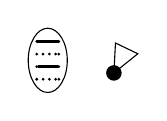
\begin{tikzpicture}[x=.4cm,y=.4cm]
\draw (0,0) ellipse (.62 and 1.02);
\foreach \y in {-.6,-.2,.2,.6}{\foreach \x in {-.35,-.15,.05,.25,.35}{\fill (\x,\y) circle (.55pt);}}
\draw[very thick] (-.35,.6)--(.35,.6) (-.32,-.2)--(.33,-.2);
\draw (2.1,-.4)--(2.15,.55)--(2.86,.21)--cycle;\fill (2.1,-.4) circle (2.8pt);
\end{tikzpicture}}

% middle, lines 13–14
Donc
\[
\begin{aligned}
\mathrm{Car}_{d*}(X)&\simeq\mathrm{trgpt}(X)\\
\mathrm{Car}_{s*}(X)&\simeq\mathrm{arc}(X)\simeq\deleted{\unsure{\mathrm{arctr}}}\mathrm{trgép}(X)\quad\text{(c'est un $\mathfrak S_3$-ens libre!)}
\end{aligned}
\]

% middle left, by second equivalence
\figure{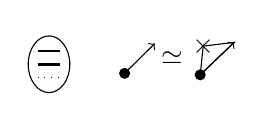
\begin{tikzpicture}[x=.48cm,y=.48cm]
\draw (0,0) ellipse (.55 and .75);\draw[thick] (-.3,.36)--(.3,.36);\draw[very thick] (-.3,0)--(.3,0);\draw[dotted] (-.3,-.36)--(.3,-.36);
\fill (2,-.24) circle (2pt);\draw[->] (2,-.24)--(2.8,.55);\node at (3.25,.17) {$\simeq$};\draw (4,-.28)--(4.08,.48)--(4.9,.58)--cycle;\draw[->] (4,-.28)--(4.9,.58);\node at (4.08,.48) {$\times$};\fill (4,-.28) circle (2pt);
\end{tikzpicture}}

% lower middle, lines 15–17
d'où
\[
C_{r'}(X)\simeq\text{ens des couples d'un trièdre et d'un triangle sécants dans $X$}
\]

% left, by Cr′
\figure{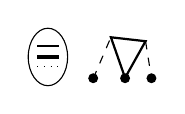
\begin{tikzpicture}[x=.5cm,y=.5cm]
\draw (0,0) ellipse (.5 and .73);\draw[thick] (-.27,.27)--(.27,.27);\draw[very thick] (-.27,0)--(.27,0);\draw[dotted] (-.27,-.25)--(.27,-.25);
\draw[thick] (1.6,.5)--(2.48,.4)--(1.96,-.53)--cycle;\draw[dashed] (1.15,-.55)--(1.6,.5) (2.48,.4)--(2.63,-.54);\foreach \x in {1.15,1.96,2.63}{\fill (\x,-.54) circle (1.8pt);}
\end{tikzpicture}}

% lower, lines 18–19
Enfin
\[
C_r(X)\simeq\text{épinglages du pavé}
\]

% lower left, by Enfin
\figure{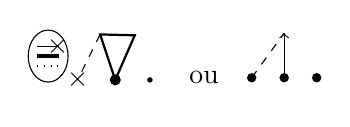
\begin{tikzpicture}[x=.55cm,y=.55cm]
\draw (0,0) ellipse (.46 and .6);\draw (-.25,.23)--(.25,.23);\node at (.22,.23){$\times$};\draw[very thick] (-.25,0)--(.25,0);\draw[dotted] (-.25,-.23)--(.25,-.23);
\draw[thick] (1.2,.5)--(2,.48)--(1.55,-.55)--cycle;\draw[dashed] (1.2,.5)--(.68,-.55);\node at (.68,-.55){$\times$};\fill (1.55,-.55) circle (2pt) (2.35,-.55) circle (1pt);
\node at (3.6,-.5) {ou};\draw[dashed] (4.7,-.5)--(5.45,.53);\draw[->] (5.45,-.5)--(5.45,.53);\foreach \x in {4.7,5.45,6.2}{\fill (\x,-.5) circle (1.7pt);}
\end{tikzpicture}}

% right margin, sideways covering diagram
% margin note written sideways
\diagram{\begin{tikzcd}[ampersand replacement=\&,column sep=large,row sep=large,cells={font=\scriptsize}]
{\substack{\mathrm{Hex}_d\\(\simeq\mathrm{tria}'\simeq\mathrm{pav}+\mathrm{ab})}}\arrow[d,"3"']\&{\substack{\mathrm{Hex}_s\simeq\mathrm{hex}\\\simeq\mathrm{tria}}}\arrow[l,"2"']\arrow[d,"3"]\&\\
{\substack{\mathrm{Hex}\\(\simeq\mathrm{pav})}}\arrow[d,"3"']\&{\substack{\mathrm{Hex}_{\mathrm{tr}}\\(\simeq\mathrm{pavcoor})\\\simeq\mathrm{trtria}}}\arrow[l,"2"']\&\\
\mathrm{triHex}\&\mathrm{Hex}_{s*}\arrow[uul,"2"]\arrow[d,"3"]\&\mathrm{Hex}_{\text{ép}}\arrow[l,dash,"\unsure{2}"']\arrow[uul,"2"]\arrow[d,"3"]\\
\&{\substack{\mathrm{Hex}_{\mathrm{tr}*}\\\text{(triples de bases}\\\text{en position particulière)}}}\arrow[uul,"2"]\&\mathrm{Hex}_{\mathrm{tror}}\arrow[l,"2"']\arrow[uul,"2"]
\end{tikzcd}}

% foot, left scribbled sketch
\figure{
\begin{tikzpicture}[scale=.48]
\foreach \x in {0,.45,.9}{\foreach \y in {0,.51,1.02}{\fill (\x,\y) circle (1.2pt);}}
\fill (0,1.02) circle (2.5pt);\node at (.65,1.02) {$\times$};
\foreach \k in {0,.25,.5,.75}{\draw (-.13,\k)--(.7,{\k+.5})--(.03,\k);}
\end{tikzpicture}}

% foot, lines 20–22
\unsure{et|alors}\quad $C_\omega(X)=\unsure{C_{r'}(X)}/\mathrm{opp}$ \deleted{\unsure{au lieu}} \inserted{$\mathrm{opp}=$} passage d'un couple d'un trièdre et triangle sécants, au couple opposé.

% archive sheet number: 82
